\section{流形的定义}
\label{sec:mfd-definition}

曲线和曲面在微积分里常由参数化给出：圆是$\theta\mapsto(\cos\theta,\sin\theta)$的像，球面可以用经纬度参数化。参数化把一块欧氏区域送到对象上；反过来读，就是用几个实数记录对象上的一个点。图~\ref{fig:mfd-latlong}说明一张参数化通常只能照顾一部分，所以我们需要多张局部记录，并规定它们在重叠处怎样换算。

\subsection{坐标图与光滑相容性}
\label{sec:mfd-charts-compatibility}

先看圆周
\[
S^1=\{\bm y\in\mathbb R^2:\lVert\bm y\rVert_2=1\}.
\]
角度$\theta$可以记录圆上的点，但取值范围必须选一个长度为$2\pi$的开区间，否则同一点会有两个角度。取$(-\pi,\pi)$时，点$(-1,0)$没有角度；取$(0,2\pi)$时，点$(1,0)$没有角度。

为什么不用半开区间$[-\pi,\pi)$把漏掉的点补上？因为那样记录就不连续了：从下方逼近$(-1,0)$的点，角度趋于$-\pi$；从上方逼近的点，角度趋于$\pi$。圆上挨得很近的两点，记录却相距接近$2\pi$。单个角度无论怎样选，不是漏点就是断开，必须用至少两张局部记录才能覆盖整个圆。

\paragraph{坐标图与图册}
把“局部记录”说准确。它应当做两件事：把一块区域一一对应到欧氏空间的开集，并且不破坏邻近关系。这正是同胚的要求，即连续的双射且逆映射也连续。于是坐标接近当且仅当点接近，上面半开区间的毛病被排除在外。

\begin{definition}[坐标图与图册]
\label{def:mfd-chart}
设$M$是拓扑空间，$n\geq0$为整数。若$U\subseteq M$是开集，$\varphi:U\to\widehat U$是从$U$到某个开集$\widehat U\subseteq\mathbb R^n$的同胚，则称$(U,\varphi)$为$M$的一张$n$维\term{坐标图}（chart），$U$为它的定义域。对$p\in U$，称
\begin{equation}
\varphi(p)=(x_1(p),\ldots,x_n(p))
\label{eq:mfd-chart-coordinates}
\end{equation}
为$p$在这张图中的坐标，实值函数$x_i:U\to\mathbb R$称为坐标函数。定义域覆盖$M$的一族坐标图称为\term{图册}（atlas）。
\end{definition}

这些名词就是地图册的术语。表~\ref{tab:mfd-atlas-analogy}列出对应关系。类比在一处需要小心：真实的地图印在纸上有边缘和比例尺，坐标图只保证拓扑上的忠实，既不保持距离也不保持角度。距离要等到第~\ref{chap:riemannian-geometry}章选定度量之后才有意义。

\begin{BookInlineTable}
  \centering
  \begin{tabular}{ll}
    \toprule
    地图册 & 流形\\
    \midrule
    地球表面 & 空间$M$\\
    地面上的地点 & 点$p\in M$\\
    一张地图覆盖的区域 & 开集$U\subseteq M$\\
    把地点标到纸上的规则 & 同胚$\varphi:U\to\widehat U$\\
    地点在图上的位置 & 坐标$\varphi(p)$\\
    相邻两图的换算表 & 转移映射$\psi\circ\varphi^{-1}$\\
    \bottomrule
  \end{tabular}
  \caption{地图册与流形术语的对应。}
  \label{tab:mfd-atlas-analogy}
\end{BookInlineTable}

圆周的两张角度图组成一个图册：
\begin{equation}
\theta_1:S^1\setminus\{(-1,0)\}\to(-\pi,\pi),\qquad
\theta_2:S^1\setminus\{(1,0)\}\to(0,2\pi).
\label{eq:mfd-circle-charts}
\end{equation}
两者的逆都是$\theta\mapsto(\cos\theta,\sin\theta)$在相应区间上的限制。图的方向是“点到坐标”，参数化的方向是“坐标到点”，二者互为逆映射。图~\ref{fig:mfd-circle-charts}的(a)(b)画出了这两张图各漏掉哪一点。

\begin{BookInlineFigure}
  \centering
  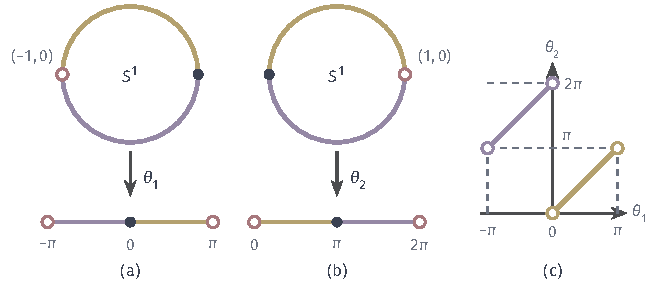
\includegraphics[width=111.605mm]{figures/04-spaces-measures-and-geometry/04-manifolds/tikz/mfd-circle-charts/figure.pdf}
  \caption{圆周的两张角度图及其转移映射。(a)(b)$\theta_1$漏掉$(-1,0)$，$\theta_2$漏掉$(1,0)$，漏掉的点用空心红圈表示。黄色弧是上半圆，紫色弧是下半圆，下方的开区间用相同颜色标出它们的坐标。(c)在重叠部分，$\theta_2$作为$\theta_1$的函数：上半圆上$\theta_2=\theta_1$（黄），下半圆上$\theta_2=\theta_1+2\pi$（紫），空心点表示这些坐标不属于重叠部分。}
  \label{fig:mfd-circle-charts}
\end{BookInlineFigure}

\paragraph{拓扑流形}
有了坐标图，就可以说一个空间“局部像$\mathbb R^n$”：每点都落在某张$n$维坐标图的定义域中。只要求这一条还不够，定义中要另加两个拓扑条件，用来排除两类病态空间。

\begin{definition}[拓扑流形]
\label{def:mfd-topological-manifold}
拓扑空间$M$称为$n$维\term{拓扑流形}（topological manifold），若它满足：
\begin{enumerate}
\item $M$是Hausdorff空间：任意两个不同点有互不相交的邻域；
\item $M$是第二可数的：拓扑有一个可数的基；
\item $M$局部欧氏：每个$p\in M$都属于某张$n$维坐标图的定义域。
\end{enumerate}
\end{definition}

Hausdorff条件保证点列的极限唯一。去掉它，就可能出现“双原点直线”：取两条实轴，把除原点以外的同名点粘在一起。所得空间每点附近都像一段实轴，局部欧氏条件成立；但两个原点没有不相交的邻域，点列$1/k$同时收敛到这两个原点。

第二可数条件排除“太大”的空间，例如不可数多条互不相交的实轴之并。这个条件有实际用途：它保证流形只有可数个连通分支，并能用一列紧集逐步穷竭，第~\ref{sec:mfd-partition-unity}节构造单位分解时就要用到。两个条件的一般讨论见第~\ref{chap:topological-spaces}章。

\paragraph{坐标变换与光滑相容}
拓扑流形只告诉我们哪些点彼此接近，还不能说一个函数“可微”。自然的想法是把函数写到坐标里再求导，但同一点可能落在两张图中，两张图的结论必须一致。这就要考察两套坐标之间的换算。

设$(U,\varphi)$与$(V,\psi)$是两张坐标图，$U\cap V\neq\varnothing$。先用$\varphi^{-1}$从第一张图回到流形上的点，再用$\psi$记到第二张图上，得到映射
\begin{equation}
\psi\circ\varphi^{-1}:\varphi(U\cap V)\to\psi(U\cap V).
\label{eq:mfd-transition}
\end{equation}
它把同一点在第一张图中的坐标换成第二张图中的坐标，称为\term{坐标变换}（transition map），也叫转移映射。

图~\ref{fig:mfd-chart-transition}画出了这个过程。要留意的是：$\varphi$和$\psi$的定义域在流形上，流形上一般没有微积分；而转移映射的定义域和值域都在欧氏空间里，可以用多元微积分判断它是否可微。这就是定义光滑结构的切入点。

\begin{BookInlineFigure}
  \centering
  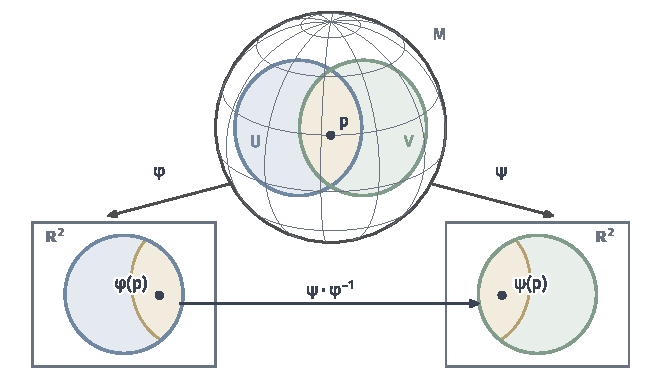
\includegraphics[width=112mm]{figures/04-spaces-measures-and-geometry/04-manifolds/matplotlib/mfd-chart-transition/figure.pdf}
  \caption{两张坐标图与转移映射。上方是球面上的两个球冠$U$（蓝）和$V$（绿），重叠部分为黄色。下方分别是向球冠中心切平面作正交投影得到的两张图。黄色区域是同一块重叠部分在两张图中的像，形状不同；转移映射$\psi\circ\varphi^{-1}$在两个黄色区域之间换算同一点$p$的坐标。}
  \label{fig:mfd-chart-transition}
\end{BookInlineFigure}

\begin{definition}[光滑相容与光滑结构]
\label{def:mfd-smooth-structure}
两张$n$维坐标图$(U,\varphi)$与$(V,\psi)$称为\term{光滑相容}（smoothly compatible）的，若$U\cap V=\varnothing$，或者坐标变换$\psi\circ\varphi^{-1}$与其逆$\varphi\circ\psi^{-1}$都是无穷次连续可微的。任意两张图都光滑相容的图册称为光滑图册。若一个光滑图册包含了所有与它的每张图都光滑相容的坐标图，就称它为极大光滑图册，也称$M$上的一个\term{光滑结构}（smooth structure）。带有光滑结构的拓扑流形称为\term{光滑流形}（smooth manifold）。
\end{definition}

本书说“光滑”都指无穷次连续可微。定义要求转移映射和它的逆都光滑，因为一个方向光滑不能保证另一方向也光滑，稍后的$x\mapsto x^3$就是例子。

极大图册听起来很大，实际使用时只需给出一个光滑图册：所有与它光滑相容的坐标图放在一起，就是包含它的唯一极大图册。需要检查的是这些新加入的图彼此也光滑相容。设$(V_1,\psi_1)$与$(V_2,\psi_2)$都与原图册相容，$q\in V_1\cap V_2$，取原图册中包含$q$的图$(U,\varphi)$。在$\psi_1(q)$附近可以经由$\varphi$中转：
\[
\psi_2\circ\psi_1^{-1}=(\psi_2\circ\varphi^{-1})\circ(\varphi\circ\psi_1^{-1}).
\]
右端两个因子都光滑，所以左端在$\psi_1(q)$附近光滑。光滑性是局部性质，逐点成立就在整个重叠区域成立。今后说“$M$的坐标图”，都指光滑结构中的坐标图。

\paragraph{例子：圆周}
现在把定义在圆周上走一遍。重叠区域是去掉$(\pm1,0)$后的两段开半圆。在上半圆，两个角度取值相同；在下半圆，$\theta_1$取$(-\pi,0)$中的值，$\theta_2$取$(\pi,2\pi)$中的值，二者相差$2\pi$。所以
\begin{equation}
\theta_2\circ\theta_1^{-1}(s)=
\begin{cases}
s, & s\in(0,\pi),\\
s+2\pi, & s\in(-\pi,0).
\end{cases}
\label{eq:mfd-circle-transition}
\end{equation}
图~\ref{fig:mfd-circle-charts}(c)是这个函数的图像，两段都是斜率为$1$的线段。

式~\eqref{eq:mfd-circle-transition}的定义域由两个不相交的开区间组成，在每段上都是平移，所以光滑，它的逆也是平移。于是这两张图构成光滑图册。坐标在下半圆跳过$2\pi$，只是记录方式的变化，圆本身并没有在那里断开。图中两段线段之间的空隙对应$\theta_1=0$，那里是$(1,0)$，它不在$\theta_2$的定义域内，所以不属于重叠部分。

\paragraph{例子：球面}
单位球面$S^2=\{\bm y\in\mathbb R^3:\lVert\bm y\rVert_2=1\}$上最方便的两张图来自\term{球极投影}（stereographic projection）。记北极$N=(0,0,1)$、南极$S=(0,0,-1)$。从北极向球面上的点$\bm y$作射线，射线与赤道平面的交点就是$\bm y$的坐标，如图~\ref{fig:mfd-stereographic}(a)所示。

下面把这个几何作图写成公式。过$N$和$\bm y$的直线上的点是$N+t(\bm y-N)$，它的第三个分量是$1+t(y_3-1)$。令第三个分量为零，得到
\[
t=\frac{1}{1-y_3}.
\]
代回前两个分量，得到北极图
\begin{equation}
\sigma_N(\bm y)=\frac{(y_1,y_2)}{1-y_3},\qquad \bm y\in S^2\setminus\{N\}.
\label{eq:mfd-stereographic-north}
\end{equation}

\begin{BookInlineFigure}
  \centering
  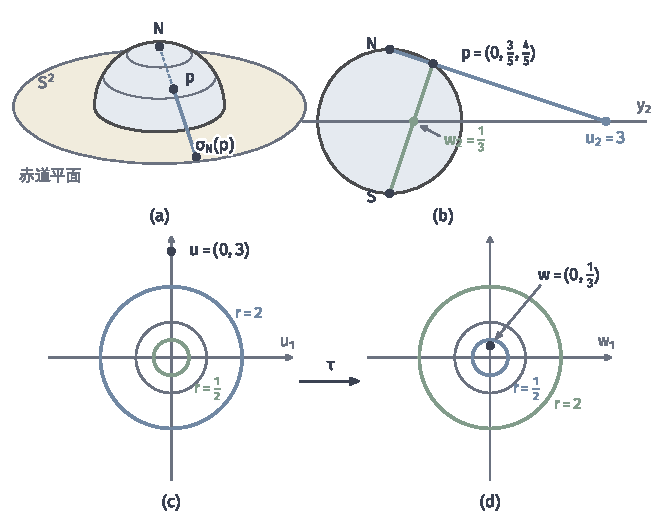
\includegraphics[width=112mm]{figures/04-spaces-measures-and-geometry/04-manifolds/matplotlib/mfd-stereographic/figure.pdf}
  \caption{球极投影及其转移映射。(a)从北极$N$过球面点$p$的射线交赤道平面（黄）于$\sigma_N(p)$，球内部分用虚线。(b)过$N$和$p=(0,\tfrac35,\tfrac45)$的竖直截面，蓝线给出北极图坐标$u_2=3$，绿线从南极给出南极图坐标$w_2=\tfrac13$。(c)(d)转移映射$\tau$把$\bm u$平面的圆周送到$\bm w$平面：半径$2$的蓝圆变成半径$\tfrac12$，半径$\tfrac12$的绿圆变成半径$2$，单位圆不变，$(0,3)$变成$(0,\tfrac13)$。}
  \label{fig:mfd-stereographic}
\end{BookInlineFigure}

反过来，给定$\bm u\in\mathbb R^2$，求球面上的对应点。记$\rho=\lVert\bm u\rVert_2^2$，点$\sigma_N^{-1}(\bm u)$在从$N$到$(\bm u,0)$的线段上，形如$(s\bm u,1-s)$。它在球面上，于是
\[
s^2\rho+(1-s)^2=1 .
\]
展开后约去$s\neq0$，得到$s(\rho+1)=2$。把$s=2/(\rho+1)$代回，就得到
\begin{equation}
\sigma_N^{-1}(\bm u)=\frac{\bigl(2u_1,\;2u_2,\;\rho-1\bigr)}{\rho+1},\qquad \rho=\lVert\bm u\rVert_2^2 .
\label{eq:mfd-stereographic-inverse}
\end{equation}
这是有理函数，$\sigma_N$与它的逆都连续，所以$\sigma_N$是$S^2\setminus\{N\}$到整个$\mathbb R^2$的同胚。同样地，从南极投影得到南极图
\begin{equation}
\sigma_S(\bm y)=\frac{(y_1,y_2)}{1+y_3},\qquad \bm y\in S^2\setminus\{S\}.
\label{eq:mfd-stereographic-south}
\end{equation}

两张图的重叠区域是去掉两极的球面，对应北极图中的$\mathbb R^2\setminus\{\bm0\}$。把式~\eqref{eq:mfd-stereographic-inverse}代入$\sigma_S$，先算分母：
\[
1+y_3=1+\frac{\rho-1}{\rho+1}=\frac{2\rho}{\rho+1}.
\]
前两个分量是$2\bm u/(\rho+1)$，相除后$\rho+1$消去，得到转移映射
\begin{equation}
\tau(\bm u)=\sigma_S\circ\sigma_N^{-1}(\bm u)=\frac{\bm u}{\lVert\bm u\rVert_2^2},\qquad \bm u\neq\bm 0.
\label{eq:mfd-stereographic-transition}
\end{equation}
这个映射叫反演：方向不变，半径变成倒数，图~\ref{fig:mfd-stereographic}(c)(d)就是它的样子。

$\tau$在$\mathbb R^2\setminus\{\bm0\}$上光滑，因为它是分母不为零的有理函数。再算$\tau\circ\tau$。由范数的计算，
\[
\lVert\tau(\bm u)\rVert_2^2=\frac{1}{\lVert\bm u\rVert_2^2},
\]
所以$\tau(\tau(\bm u))=\bm u$，$\tau$的逆就是它自己，同样光滑。于是$\{\sigma_N,\sigma_S\}$是$S^2$的光滑图册。球面作为$\mathbb R^3$的子空间，Hausdorff性与第二可数性都从$\mathbb R^3$继承，因此是二维光滑流形。

\paragraph{例子：欧氏开集与乘积}
最简单的光滑流形是$\mathbb R^n$本身，用恒等映射作唯一的图。它的任意开子集$W$也是光滑流形，图为恒等映射在$W$上的限制。更一般地，光滑流形的开子集用原有坐标图限制到其中，就成为同维光滑流形。

两个流形可以相乘。设$M$与$N$分别是$m$维与$n$维光滑流形，$(U,\varphi)$与$(V,\psi)$分别是二者的坐标图，令
\begin{equation}
(\varphi\times\psi)(p,q)=(\varphi(p),\psi(q))\in\mathbb R^{m+n}.
\label{eq:mfd-product-chart}
\end{equation}
这些乘积图覆盖$M\times N$。两张乘积图之间的坐标变换是两个坐标变换并排作用，各自光滑，所以并排后也光滑。乘积拓扑仍是Hausdorff且第二可数的，于是$M\times N$是$m+n$维光滑流形，称为\term{乘积流形}（product manifold）。

\term{环面}（torus）$T^2=S^1\times S^1$是最常用的乘积例子。一点由两个角度$(\theta,\phi)$记录，图~\ref{fig:mfd-torus-product}左边的正方形就是角度的取值范围，右边是同一个流形放进$\mathbb R^3$的样子，公式为
\[
\bigl((2+r\cos\phi)\cos\theta,\ (2+r\cos\phi)\sin\theta,\ r\sin\phi\bigr),\quad 0<r<2 .
\]
这只是外观，环面作为乘积流形并不需要$\mathbb R^3$。正方形的上下边是同一个圆，左右边也是同一个圆，把两组对边粘起来就得到环面。

\begin{BookInlineFigure}
  \centering
  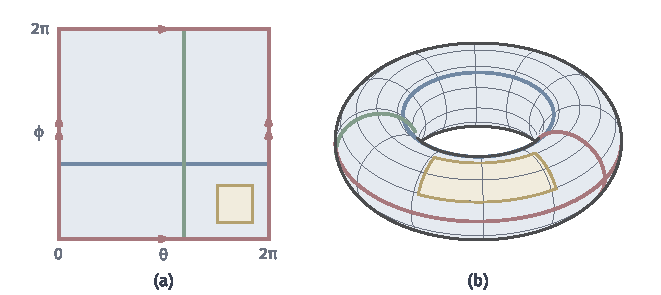
\includegraphics[width=112mm]{figures/04-spaces-measures-and-geometry/04-manifolds/matplotlib/mfd-torus-product/figure.pdf}
  \caption{环面$S^1\times S^1$的角度坐标。(a)角度正方形，带箭头的红色对边两两等同；黄色矩形是一小块坐标区域，蓝线$\phi=$常数，绿线$\theta=$常数。(b)嵌入$\mathbb R^3$的环面（$r=0.82$）上同一块区域和同样两条圈，红色两条圈是$\phi=0$和$\theta=0$的接缝。灰线为角度网格。}
  \label{fig:mfd-torus-product}
\end{BookInlineFigure}

圆周的两张图做乘积，就得到环面的四张图：$\theta_a\times\theta_b$，$a,b\in\{1,2\}$。以圆周上$\theta_1=1$和$\theta_1=-2$对应的两点组成的乘积点为例，它在四张图中的坐标分别是
\[
(1,-2),\quad (1,-2+2\pi),\quad (1,-2),\quad (1,-2+2\pi),
\]
依次对应$(a,b)=(1,1),(1,2),(2,1),(2,2)$，其中第一个角度$1\in(0,\pi)$两图相同，第二个角度$-2\in(-\pi,0)$需要加$2\pi$。这正是式~\eqref{eq:mfd-circle-transition}在两个分量上分别作用。

\paragraph{相容性是附加的选择}
光滑相容不是自动成立的。在$\mathbb R$上，$\chi(x)=x^3$是$\mathbb R$到$\mathbb R$的同胚，因而是一张合法的拓扑坐标图。它与恒等图之间的两个转移映射是
\[
\chi\circ\mathrm{id}^{-1}(x)=x^3,\qquad \mathrm{id}\circ\chi^{-1}(y)=y^{1/3}.
\]
前者光滑，后者在原点不可微。所以$\chi$与恒等图不光滑相容。

$\{\chi\}$单独也是一个光滑图册，它决定了$\mathbb R$上另一个光滑结构。在这个结构下，函数$f(x)=x$的坐标表示是$f\circ\chi^{-1}(y)=y^{1/3}$，不再光滑。可见同一个拓扑空间上的光滑性取决于所选的光滑结构。后文默认使用标准结构，两种结构之间能否用光滑映射互相转换，留到第~\ref{chap:manifold-relations}章讨论。

\paragraph{维数}
定义中的$n$对每张图都相同。假如允许不同维数的图，光滑情形也不会出现矛盾。设$m$维与$n$维的两张图重叠，$\tau$是转移映射，$\tau^{-1}$是逆，对$\tau^{-1}\circ\tau=\mathrm{id}$和$\tau\circ\tau^{-1}=\mathrm{id}$用链式法则，得到
\[
\bm J_{\tau^{-1}}\bm J_{\tau}=\bm I_m,\qquad
\bm J_{\tau}\bm J_{\tau^{-1}}=\bm I_n .
\]
一个$n\times m$矩阵既有左逆也有右逆，就是可逆方阵，所以$m=n$。多元链式法则可参考\BookChapterRef{chap:multivariate-differentiation}{卷二第17章“多元函数微分”}。对拓扑流形，同样的结论依赖区域不变性定理，证明需要代数拓扑的工具，篇幅较长，这里只使用结论。

\subsection{带边界的流形}
\label{sec:mfd-boundary}

闭圆盘
\[
\overline{B}{}^2=\{\bm y\in\mathbb R^2:\lVert\bm y\rVert_2\leq1\}
\]
不是上面意义的流形：圆周上的点无论取多小的邻域，邻域都只在圆盘一侧，形状是半个圆盘，而不是一个开圆盘。区间$[0,1]$的端点、半球面的赤道也是这样。这些对象并不病态，只是局部模型要放宽：从欧氏开集放宽到半空间。

\paragraph{半空间模型}
记$n\geq1$维闭上半空间及其边界为
\begin{equation}
\mathbb H^n=\{\bm x\in\mathbb R^n:x_n\geq0\},\qquad
\partial\mathbb H^n=\{\bm x\in\mathbb R^n:x_n=0\}.
\label{eq:mfd-halfspace}
\end{equation}
$\mathbb H^n$的开子集指它与$\mathbb R^n$中某个开集的交。例如半圆盘$\{\bm x\in\mathbb H^2:\lVert\bm x\rVert_2<1\}$含有底边上的点，它是$\mathbb H^2$的开子集，却不是$\mathbb R^2$的开集。

图~\ref{fig:mfd-boundary-models}比较了三种局部情形。内点(a)的邻域是开圆盘，模型是$\mathbb R^2$的开集；边界点(b)的邻域是半个圆盘，模型是$\mathbb H^2$的开子集；正方形的角点(c)的邻域在平面坐标中是象限，不在这两种模型之内，后面专门讨论。

\begin{BookInlineFigure}
  \centering
  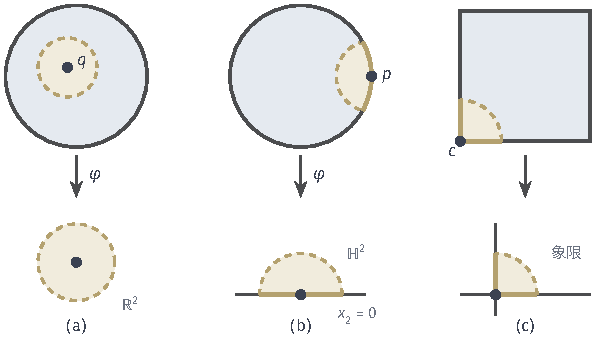
\includegraphics[width=100.856mm]{figures/04-spaces-measures-and-geometry/04-manifolds/tikz/mfd-boundary-models/figure.pdf}
  \caption{三种局部模型。上排是闭圆盘或闭正方形中的一个小邻域（黄），下排是它在坐标图中的像。(a)内点$q$的邻域对应$\mathbb R^2$的开圆盘，虚线表示边不含在内。(b)边界点$p$的邻域对应$\mathbb H^2$的半圆盘，粗黄线是位于边界上的部分，含在邻域内。(c)角点$c$的邻域在平面坐标中是象限，不是半圆盘。}
  \label{fig:mfd-boundary-models}
\end{BookInlineFigure}

\begin{definition}[带边界的拓扑流形]
\label{def:mfd-manifold-with-boundary}
Hausdorff且第二可数的拓扑空间$M$称为$n$维\term{带边界流形}（manifold with boundary），若每个$p\in M$都有开邻域$U$和从$U$到$\mathbb H^n$的某个开子集的同胚$\varphi$。若某张这样的图把$p$送到$\partial\mathbb H^n$中，称$p$为\term{边界点}（boundary point）；若某张图把$p$送到$\{x_n>0\}$中，称$p$为内点。全部边界点组成的集合记为$\partial M$。
\end{definition}

$\{x_n>0\}$本身是$\mathbb R^n$的开集，所以内点附近的局部模型与无边界情形相同。没有边界点的带边界流形就是前面的流形，为了区分，后者也称无边界流形。

\paragraph{半空间上的光滑性}
要定义带边界流形的光滑结构，先得说清半空间开子集上的映射何时光滑。边界点处只有一侧的值，双侧差商算不了偏导数。约定的做法是借助延拓：若映射在边界点附近能光滑地延拓到一个完整的欧氏开邻域，就称它在那里光滑。

\begin{definition}[半空间开子集上的光滑映射]
\label{def:mfd-smooth-halfspace}
设$A\subseteq\mathbb H^n$是开子集，$F:A\to\mathbb R^k$。若对每个$\bm a\in A$，都有$\mathbb R^n$中的开邻域$W\ni\bm a$与光滑映射$\widetilde F:W\to\mathbb R^k$，使$\widetilde F=F$在$W\cap A$上成立，则称$F$光滑。
\end{definition}

延拓不唯一，但边界点处各阶导数与延拓的选择无关。原因在于内点可以逼近边界点：任意边界点$\bm a$都是内点$\bm a+t\bm e_n$（$t\to0^+$）的极限，延拓在这些内点处的导数就是$F$本身的导数，而$\widetilde F$的各阶导数连续，所以在$\bm a$处的值等于内侧导数的极限，由$F$决定。

有了这一定义，带边界流形的光滑相容性、光滑图册和光滑结构可以逐字照搬定义~\ref{def:mfd-smooth-structure}，只是把坐标变换理解为$\mathbb H^n$开子集之间的映射。

\paragraph{内点与边界点不会混淆}
定义~\ref{def:mfd-manifold-with-boundary}说的是“某张图”把点送到边界，于是要问：会不会有一点在一张图中是边界点，在另一张中是内点？直观上，内点四周都有路可走，边界点只有一侧。下面用Jacobian矩阵把这个直观变成证明。

\begin{theorem}[边界点的坐标无关性]
\label{thm:mfd-boundary-invariance}
设$M$是光滑带边界流形，$p\in M$。若某张光滑坐标图把$p$送到$\partial\mathbb H^n$中，则每张包含$p$的光滑坐标图都把$p$送到$\partial\mathbb H^n$中。
\end{theorem}

\begin{proof}
用反证法。设图$(V,\psi)$把$p$送到边界，图$(U,\varphi)$把$p$送到$\{x_n>0\}$。取$\varphi(p)$在$\mathbb R^n$中的开球$W$，使$W\subseteq\varphi(U\cap V)$，这一步用到$\varphi(p)$是内点。记$\tau=\psi\circ\varphi^{-1}$，它在$W$上光滑。

它的逆$\varphi\circ\psi^{-1}$在$\psi(p)$附近光滑，即在$\psi(p)$的欧氏邻域上有光滑延拓$\widetilde\tau$。在$\varphi(p)$附近，$\widetilde\tau\circ\tau=\mathrm{id}$，对它求导得到
\[
\bm J_{\widetilde\tau}(\psi(p))\,\bm J_\tau(\varphi(p))=\bm I_n .
\]
于是$\bm J_\tau(\varphi(p))$可逆。

由局部反函数定理，$\tau$把$\varphi(p)$的某个开邻域映成$\psi(p)$在$\mathbb R^n$中的一个开邻域，该定理可参考\BookChapterRef{chap:implicit-inverse-functions}{卷二第19章“隐函数与反函数”}。可是$\tau$的值都在$\mathbb H^n$中，而$\psi(p)$的最后一个坐标为零，它的任何欧氏开邻域都含有$x_n<0$的点。这一矛盾说明假设不成立。
\end{proof}

对拓扑带边界流形，同样的结论也成立，但证明需要同调等工具，读者可查阅代数拓扑的教材。今后谈论$\partial M$时，总是在光滑情形下进行。

\paragraph{边界本身的结构}
边界点处的坐标图限制到边界上，给出边界的局部坐标。设$(U,\varphi)$是包含边界点的图，由定理~\ref{thm:mfd-boundary-invariance}，
\[
\varphi(U\cap\partial M)=\varphi(U)\cap\partial\mathbb H^n .
\]
把$\partial\mathbb H^n$等同于$\mathbb R^{n-1}$，限制映射$\varphi|_{U\cap\partial M}$就是$\partial M$的一张$n-1$维坐标图。两张这样的图之间的坐标变换是原坐标变换在边界上的限制，仍然光滑。所以$\partial M$是$n-1$维无边界光滑流形。

用闭圆盘检验这些定义。内部的点用平面坐标的限制作图。边界点用极坐标$(\theta,s)$作图，其中$s=1-r\geq0$，例如在$(1,0)$附近取
\[
\theta\in(-\tfrac{\pi}{2},\tfrac{\pi}{2}),\qquad s\in[0,\tfrac12).
\]
在这张图中，圆周恰好对应$s=0$，所以$\partial\overline B{}^2=S^1$，它是一维无边界流形。区间$[0,1]$是一维带边界流形，边界由两个端点组成，是零维流形。

\paragraph{角点不是同一种光滑边界}
闭正方形$[0,1]^2$同胚于闭圆盘，所以是拓扑带边界流形。但在角点处，平面坐标给出的局部模型是象限$\{x_1\geq0,x_2\geq0\}$，而不是半平面。

能否换一张图把象限摊平？把平面看作复平面，$z\mapsto z^2$确实把象限映成上半平面。可它的逆$z\mapsto\sqrt z$在原点不可微，所以这样得到的坐标与平面原有坐标不光滑相容。这说明如果沿用平面坐标所定义的光滑性，角点不能纳入光滑带边界流形的框架。这类对象需要另行建立带角流形的理论，本书不作讨论。
